\chapter{Reactive Component Language\label{language}}

\begin{quote}
In theory, there is no difference between theory and practice. \linebreak
But, in practice, there is.  \emph{Anonymous}
\end{quote}

In this chapter, we present a programming language for reactive components.
We state the motivation for the language, our assumptions for tractability, and the features that guided our design.
We then show how reactive components are expressed in the language and we conclude with illustrative examples.

\section{Motivation}

An implementation of reactive components is necessary for at least three reasons.
First and foremost, an implementation tests the practicality of the model.
The act of implementing the model will reveal whether the assumptions upon which the model is founded can be realized using existing techniques.
Conversely, an implementation can suggest restrictions to the model that are necessary to produce an effective implementation.
An example of this was seen in chapter~\ref{model} where the component instance was used as proxy for its state variables for the purpose of determining which variables were involved in a transaction.
Implementation forces one to supply and consider details that can either qualify or disqualify a model as a practical engineering tool.
This is consistent with the emerging attitude in systems research that all new ideas and techniques must be accompanied by relevant tools and evaluations to show their feasibility.

Second, language support for a model is beneficial because it closes the semantic gap between reasoning and implementation.
The importance of language support can be seen in techniques like structured programming~\cite{dahl1972structured} and object-oriented programming~\cite{booch1982object}.
While these techniques can be applied in virtually any setting, their lasting utility is derived from their implementation in a variety of programming languages.
Providing language support for a model raises the level of abstraction and allows reasoning about a system directly from its specification instead of reasoning in one set of semantics while implementing in another which can be tedious and error-prone.
Language support allows developers to rely on the consistent application of the semantics of the model through strict enforcement, e.g., checking by a compiler.

Third, an implementation is necessary to demonstrate that the model can be applied successfully to real-world design and implementation problems.
That is, given a platform for reactive components, we can design, construct, and evaluate systems based on the reactive component paradigm.
Furthermore, we can evaluate critically the design and implementation processes that the model and platform encourage.
By comparing implementations of similar systems in two different models, we can gain insight into the strengths and weaknesses of the model.
These ideas will be explored further in chapter~\ref{evaluation}.

\section{Approach}
Our approach to implementing reactive components is to define a programming language for reactive components and implement that language in an interpreter.
The Go programming language~\cite{go} was adopted as the \emph{transformational basis} of the language due to its simplicity.
That is, we will defer to Go's syntax and semantics for types,declarations, statements, and expressions when they are not in conflict with the semantics of reactive components.
Go is an imperative programming language that supports methods but places no emphasis on an inheritance hierarchy.
In the same vein, Go does not have constructors, destructors, function overloading, and operator overloading.
Go's type system is straightforward and the syntax of expressions and statements resemble C.
This combination, in our opinion, makes Go an attractive transformational basis in terms of being tractable in implementation and approachable by a general audience.
We will not discuss the syntax and semantics of Go except when they interact with the semantics of reactive components.
Our implementation of Go is intentionally incomplete as a full implementation is beyond the scope of this project.

The choice to implement an interpreter instead of a byte-code interpretation, i.e., a virtual machine, or a compiler made the task tractable as it avoids code generation, linking, and loading.
However, in moving from the interpreter to a compiler, the processes of code generation, linking, and loading must provide certain guarantees.
We describe the challenges of moving from interpreter to compiler in chapter~\ref{future_work}.

\paragraph{Static system assumption.}
To make implementation tractable, we will assume that the systems to be implemented have a static topology meaning that all reactive components are statically allocated.
Both finite state and infinite state (subject to system resource limits) reactive components are permitted, but both the number and configurations of reactive components in a system are fixed.
This is equivalent to systems that assume a fixed number of actors and is roughly equivalent to systems that assume a fixed number of threads.
These assumptions are common in embedded and real-time systems due to the combination of limited resources and a need for predictability.
We also believe these assumptions are common in less constrained environments as the number of threads is often fixed by the design, e.g., only a fixed number of concurrent activities is needed, or the number of threads is limited by the number of available physical cores.
Thus, even with the static system assumption, an implementation of the model is still applicable to many systems of interest.
We leave implementation of extensions that facilitate the dynamic creation and binding of reactive components for future work.

\paragraph{Efficient communication.}
One of the goals of the implementation was to allow components to communicate efficiently.
There are three modes by which a component (sender) can share information with another component (receiver) as they interact through push ports and pull ports.
First, the sender may use \emph{value semantics} where it provides a complete copy of the value to be communicated.
This approach is reasonable for values like numbers and small records.
Second, a sender may use \emph{reference semantics} where it provides a pointer (reference) to the data to be communicated.
The approach is reasonable when the sender offers up a large data structure.
The receiver is responsible for copying any data that needs to be retained.
When using reference semantics, receivers may read the data structure represented by the pointer but may not alter or remember the original data structure in any way.
Third, a sender may use \emph{move semantics} where it provides a pointer to a data structure that the receiver may adopt as its own.
In this case, the sender promises to ``forget'' the data structure as the receiver is the new owner of the data structure.
Move semantics are appropriate when the size of the data to be communicated is large, there is a single receiver, and the sender does not need to retain the data.
These conditions arise is situations like network stacks and pipelines.

\paragraph{Memory model.}
A value is allocated in either the constant segment, a stack, the component segment, or a heap.
The constant segment is used to store aggregate literals like string constants.
Function parameters and local variables are allocated on a call stack as they are in C or C++.
The component segment contains statically allocated components.
The set of addresses $A$ containing the state of a component is the transitive closure of a points-to relation starting from the pointer to the component $c$.
Assuming statically allocated components, the set of addresses $pointsto(c)$ all reside in component space.
The set of addresses $H = A \setminus pointsto(c)$ constitute a heap or a set of dynamically allocated blocks of memory.
Based on the semantics of reactive components, the heaps of two different components must be disjoint.
Logically, then, each component has its own heap from which it can allocate memory.
The component segment and the heaps contain all of the mutable state in the system.
Mutable state outside of a component, e.g., a global variable, is prohibited as it may introduce a data race.

\section{Programming Language}

\paragraph{Components.}
A component resembles a \verb+struct+ in Go since it is a group of named state variables.
A component, then, is defined with the following syntax:
\begin{verbatim}
type identifier component { field list };
\end{verbatim}
For example,
\begin{verbatim}
type Clock component {
  flag bool;
  counter uint;
};
\end{verbatim}
introduces a type named \verb+Clock+ that is a reactive component with two fields (state variables).
The type of a field may be another component type to support recursive encapsulation.

\paragraph{Receivers.}
A method in Go has one of the following two forms:
\begin{verbatim}
func (identifier typeName) methodName signature body
func (identifier *typeName) methodName signature body
\end{verbatim}
The first form operates on a copy of a value of type \verb+typeName+.
The second form operates on a pointer to a value of type \verb+typeName+.
The parameter \verb+identifier+ performs the same function as the \verb+this+ keyword in C++ and Java.
The syntax \verb+(identifier typeName)+ is called a receiver and the syntax \verb+(identifier *typeName)+ is called a pointer receiver.
Many of the syntactic elements introduced for reactive components use a pointer receiver.

\paragraph{Intrinsic and dereference mutability.}
Variables and parameters may be declared with an \emph{intrinsic mutability} and a \emph{dereference mutability}.
Intrinsic mutability limits the operations that can be performed on an lvalue of the variable or parameter while dereference mutability limits the operations that can be performed on lvalues derived from the rvalue of the variable or parameter.
By default, variables and parameters have mutable intrinsic and dereference mutability.
The following code is legal and sets \verb+z+ to 6.
\begin{verbatim}
var x uint = 3;
var y *uint = &x;
var z = x + *y;
\end{verbatim}

Declaring a variable or parameter to have immutable intrinsic mutability (\verb+const+) prevents the variable or parameter from being changed after it is initialized.
The following code is illegal:
\begin{verbatim}
var x const uint = 3;
x = 4; // Illegal
\end{verbatim}
Immutable intrinsic mutability is enforced when taking the address of a variable or parameter:
\begin{verbatim}
var x const uint = 3;
var y *uint = &x;        // Illegal
var z +const *uint = &x; // Legal
var a uint = *z;         // Legal
*z = 5;                  // Illegal
\end{verbatim}
The second line is illegal because \verb+x+ could change through a statement like \verb+*y = 5;+.
The third line causes \verb+z+ to have immutable dereference mutability (\verb|+const|).
The expression \verb+*z+ can serve as an rvalue (line 4) but it cannot serve as an lvalue (line 5).

Dereference mutability is ``sticky.''
For example:
\begin{verbatim}
var x +const **uint = ...;
var y +const *uint = *x; // Legal
var z *uint = *x;        // Illegal
\end{verbatim}
The second line honors the guarantee that all of the memory accessible through \verb+x+ is immutable.
Dereference mutability is checked in assignment and calls such as normal function call, method call, port activation, and bindings.
Dereference mutability affects type from which lvalues can be derived, namely, pointers and slices (indexable pointers).
Immutable dereference mutability is one of the techniques that is used to enforce the immutable phase of state transitions.

The second kind of mutability is called \emph{foreign} mutability.
Foreign mutability is like immutable mutability with the added condition that an address with foreign mutability cannot be stored in the heap.
The primary application of foreign mutability is declaring the parameters of push ports and reactions with foreign dereference mutability.
This supports the goal of using reference semantics for communication while enforcing the isolation of heaps.
\begin{verbatim}
var x +foreign *uint = ...;
var y **uint = new *uint;
*x = 3;                            // Illegal
*y = x;                            // Illegal
var z +foreign *uint = x;          // Legal
\end{verbatim}
The third line is illegal because the lvalue given by \verb+*x+ is immutable.
The fourth line is illegal because it casts away the \verb|+foreign| of \verb+x+.
(Notice that declaring \verb+y+ with \verb|+foreign| would cause the lvalue to be immutable.)
The fifth line is legal because the lvalue is mutable and the \verb|+foreign| is preserved.
The consequence of these semantics is that variables that contain pointers that are declared \verb|+foreign| may only be stored on the stack.

%% Table~\ref{mutability} describes how the intrinsic and dereference mutability is computed for various expressions.
%% The operation of interest is the dereference operation which shows how dereference mutability is ``sticky'' and conservatively assumes that all pointers refer to an address on the heap.

The following checks are applied to assignment statements:
\begin{enumerate}
\item The lvalue and rvalue must be type compatible.
\item The lvalue must have mutable intrinsic mutability.
\item If the type involved contains a pointer or slice, check for compatible dereference mutability in table~\ref{assignmut}.
  Essentially, the dereference mutability of the lvalue must be at least as ``weak'' as the dereference mutability of the rvalue.
  This enforces the ``stickiness'' of dereference mutability.
\end{enumerate}

%% \begin{table}
%%   \centering
%%   \begin{tabular}{ccccp{1.75cm}cccc}
%%     Kind & Seg & Intrin & Deref & Op & Kind & Seg & Intrin & Deref \\
%%     \hline
%%     lvalue & S & A & B & load              & rvalue & S    & A & B \\
%%     rvalue & S & A & B & deref (\verb+*+)  & lvalue & heap & B & B \\
%%     lvalue & S & A & B & ref (\verb+&+)    & rvalue & S    & A & B \\
%%     lvalue & S & A & B & select (\verb+.+) & lvalue & S    & A & B \\
%%     lvalue & S & A & B & index (\verb+[]+) & lvalue & S    & A & B \\
%%   \end{tabular}
%%   \caption{Intrinsic and dereference mutability for various operations\label{mutability}.  The possible choices for segment are constant, stack or heap (includes the component segment).  The possible choices for the intrinsic and dereference mutability are mutable, immutable, and foreign.}
%% \end{table}

\begin{table}
  \centering
  \begin{tabular}{cccc}
              & Mutable & Immutable & Foreign \\
    Mutable   & Yes     & No        & No      \\
    Immutable & Yes     & Yes       & No      \\
    Foreign   & Yes     & Yes       & Yes     \\
    \end{tabular}
  \caption{Dereference mutability compatibility for assignment.\label{assignmut}.  The rows represent the dereference mutability of the lvalue and the columns represent the dereference mutability of the rvalue.}
\end{table}

A parameter is \emph{foreign safe} if (1) the type of the parameter does not contain pointers or slices or (2) the parameter is declared with foreign dereference immutability.
A parameter list is foreign safe if all parameters in the list are foreign safe.
A signature (a parameter list with a return parameter) is foreign safe if the parameter list and return parameter are both foreign safe.

\paragraph{Initializers.}
A initializer is used to initialize the fields of a reactive component.
This allows one to initialize components before the scheduler starts.
This is necessary for establishing invariants as is commonly done in formal models, e.g., the \verb+initially+ section of UNITY~\cite{chandy1989parallel}.
An initializer has the form:
\begin{verbatim}
init (id *typeName) initializerName signature body
\end{verbatim}
An initializer is similar to a method but has additional semantics:
\begin{itemize}
\item An initializer must have a pointer receiver to a component type.
\item The signature must be foreign safe.
\item An initializer may only be invoked by another initializer.
\item An initializer sets the heap on entry and resets the heap on exit so that all allocated memory is attributed to the receiver.
\end{itemize}

\paragraph{Instances.}
An instance is a top-level component.
An instance is declared with the following syntax:
\begin{verbatim}
instance identifier typeIdentifier initializerIdentifier (expressionList);
\end{verbatim}
For example, \verb+instance c Clock Init ();+ declares as instance named \verb+c+ of type \verb+Clock+ and will call the initializer \verb+Init+ with an empty list of arguments.
The instance identifier must be unique, the type identifier must refer to a component, and the initializer must be declared for the component type.

\paragraph{Actions.}
An action has the form:
\begin{verbatim}
action (id +const *typeName) identifier (booleanExpression) body
\end{verbatim}
The immutable dereference mutability of the receiver enforces the immutable phase of transactions.
Actions may only be defined for component types.
The Boolean expression is the precondition of the action.
The receiver variable is in scope for the evaluation of the precondition.
The body contains the state transitions associated with the action.

\paragraph{Reactions.}
A reaction has the form:
\begin{verbatim}
reaction (id +const *typeName) identifier (parameterList) body
\end{verbatim}
As with actions, the immutable dereference mutability of the receiver enforces the immutable phase of transactions.
Reaction may only be defined for component types.
The name of a reaction is used when binding.
The parameter list declares the parameters that are passed to the reaction.
The parameter list must be foreign safe.
This prevents the reaction from storing memory addresses from the component that activated the reaction.
The body contains the state transitions associated with the reaction.

\paragraph{Push ports.}
A push port is declared as a field of a component with push port type.
A push port type has the form:
\begin{verbatim}
push (parameterList)
\end{verbatim}
The parameter list declares the parameters that are passed to any bound reaction.
The parameter list must be foreign safe.
The following example declares a push port named \verb+response+ in the \verb+Clock+ component:
\begin{verbatim}
type Clock component {
  ...
  response push (t uint);
};
\end{verbatim}

\paragraph{Getters.}
A getter has the form:
\begin{verbatim}
getter (id +const *typeName) identifier signature body
\end{verbatim}
A getter is similar to a method but has additional semantics:
\begin{itemize}
\item A getter must have a pointer receiver to a component type declared with immutable dereference mutability.
\item The signature must be foreign safe.
\item A getter may only be invoked by another getter or an action or reaction in the immutable phase.
\item An getter sets the heap on entry and resets the heap on exit so that all allocated memory is attributed to the receiver.
\end{itemize}

\paragraph{Pull ports.}
A pull port is declared as a field of a component with pull port type.
A pull port type has the form:
\begin{verbatim}
pull (parameterList) returnParameter
\end{verbatim}
The parameter list declares the parameters that are passed to the bound getter.
The parameter list and return parameter must be foreign safe.
Pull ports are called like getters and place the same restriction on the caller, that is, a pull port may only be invoked by a getter or an action or reaction in the immutable phase.
The following example declares a pull port named \verb+isBufferFull+ in the \verb+Producer+ component:
\begin{verbatim}
type Producer component {
  ...
  isOutputBufferFull pull () bool;
};
\end{verbatim}
In this example, the intent of the pull port is to allow a \verb+Producer+ to interrogate the status of a down stream buffer to implement flow control.

\paragraph{Binders.}
Binders allow reactions to be associated with push ports and getters to be associated with pull ports.
Binding and recursive encapsulation are the two mechanisms for composing reactive components.
A binder has the form:
\begin{verbatim}
bind (id *typeName) identifier {
  bindStatement
  ...
}
\end{verbatim}
For example:
\begin{verbatim}
bind (this *System) TheBinder {
  this.producer.Out -> this.consumer.In;
  this.producer.isOutputBufferFull <- this.consumer.isInputBufferFull;
}
\end{verbatim}
The first statement of the example binds the \verb+Out+ push port of the \verb+System+'s \verb+producer+ to the \verb+In+ reaction of the \verb+System+'s \verb+consumer+\footnote{The select operator(\texttt{.}) acts automatically dereferences a pointer.}.
The second statement of the example binds the \verb+isOutputBufferFull+ pull port of the \verb+System+'s \verb+producer+ to the \verb+isInputBufferFull+ getter of the \verb+System+'s \verb+consumer+.
The left side of a bind statement always refers to a port while the right side refers to a getter or action.
The direction of the arrow indicates the logical flow of information.
Thus, information flows from the push port to a reaction (\verb+->+) and information flows from the getter to a pull port (\verb+<-+).
A pull port must be bound to exactly one getter.
A reaction may be bound to at most one push port.
Binders are associated with a component type and created for each instance of that component type.

\paragraph{Activations.}
Activations are the mechanism by which transactions extend to other components via push port/reaction bindings.
Activations also serve as the boundary between the immutable and mutable phases of a transaction.
An activation statement has the form:
\begin{verbatim}
activate portName (arguments) ... {
  statements
};
\end{verbatim}
Activation statements can only occur in the body of an action or a reaction.
Assume that the receiver of the action or reaction is named \verb+this+.
The expression \verb+this.portName+ must refer to a push port and the arguments passed to the push port must agree with its signature.
The list of push ports in an activate statement is optional.
When an activation statement is executed, the named push ports are activated meaning that the reactions bound to those push ports are activated with the given arguments.
This chaining of activations forms a transaction that resembles a tree where the root of the tree is a component/action pair, the other nodes are component/reaction pairs, and the links represent port activations.
Once all of the actions and reactions in the transaction have activated their last push port, they proceed to execute the body of the activate statements.
Recall that \verb+this+ has immutable dereference mutability.
Thus, all computation up to and including the last port activation constitutes the immutable phase of the transaction since the state of the components is not allowed to change.
Within the scope of the body, \verb+this+ changes to mutable dereference mutability which allows the state of a component to be changed.
Thus, the bodies of activation statements form the mutable phase of the transaction.
Actions and reactions return, i.e., the flow of control is halted, after the execution of the body of a activation statement.
Activate statements guarded by \verb+if+ statements facilitate \emph{conditional activation}.
An activate statement may not appear in another activate statement.

\paragraph{Arrays.}
A homogeneous group of sub-components may be declared using array syntax.
For example,
\begin{verbatim}
type System component {
  clock [5]Clock;
  ...
};
\end{verbatim}
declares 5 \verb+Clock+ sub-components.
To request the time from each \verb+Clock+, the \verb+System+ declares as array of 5 push ports and a \emph{dimensioned} action:
\begin{verbatim}
type System component {
  clock [5]Clock;
  push [5]request ();
  ...
};

[5] action (this +const *System) (...) {
  ...
  activate clock[IOTA] {
    ...
  };
}
\end{verbatim}
A dimensioned action is parameterized with an integral constant in the range $[0,dimension)$.
This constant is accessed through the \verb+IOTA+ symbol.
A push port in an array is activated by supplying an index.
The index expression must be constant to facilitate the check for sound composition.
Reactions may be dimensioned as well:
\begin{verbatim}
[5] reaction (this +const *System) clock (t int) { ... }
\end{verbatim}
A \verb+for+-loop over an integral range may be used to generate bindings without explicitly listing each binding.
For example:
\begin{verbatim}
bind (this *System) {
  for i ... 5 {
    this.request[i] -> this.clock[i].request;
  };
}
\end{verbatim}

\paragraph{Transferrable heaps.}
A key requirement for implementing reactive components is that the state of each component remain disjoint.
Foreign dereference mutability allows components to safely communicate with pointers because it ensures that those pointers are forgotten after the transaction.
For efficient communication, we also desire the ability to transfer a data structure (the heap) from one component (the sender) to another component (the receiver).
The sender offers the heap to its receivers and one of the receivers may claim the heap.
If the heap is accepted, the sender must forget all references to the heap.

A heap is a type so named because it resembles a heap used for dynamic memory allocation.
A heap has a distinguished root that contains the data structure that will be transferred.
A heap is entirely self-contained, that is, any pointer found in the heap may only point to an address in the heap.
This ensures that the receiver may not access state in the sender after a transfer.
Heaps may form hierarchies.

A heap is created with the \verb+new+ operator.
For example:
\begin{verbatim}
var x *heap int = new heap int;
\end{verbatim}
creates new heap with an integer root.

A \verb+change+ statement allows one to access the root of the heap.
For example:
\begin{verbatim}
change (x, y) {
  *y = 3;
};
\end{verbatim}
In the example, \verb+x+ is a pointer to a heap and \verb+y+ is a variable that points to the root of the heap.
The root variable is valid for the scope introduced by the \verb+change+ statement.
The root variable will be set to \verb+nil+ if the heap is no longer valid.
Within the scope of the \verb+change+ statement, all other variables and parameters are re-entered with foreign dereference immutability.
This enforces the isolation of heaps by preventing the heap from storing a pointer that refers to a location in another heap.

Heaps are treated like a stack.
On entering an action or reaction, the stack of heaps contains a single heap:  the heap associated with the component.
A \verb+change+ statement pushes a new heap on the stack.
All memory allocations are performed using the current heap.

A \verb+move+ expression allows a receiver to take ownership of a heap being offered by a sender.
For example:
\begin{verbatim}
var z *heap int = move (x);
\end{verbatim}
If \verb+x+ refers to a heap that has already been moved, i.e., claimed by this component or another component, then the result of the \verb+move+ is a \verb+nil+ pointer.
A \verb+change+ statement can be used to access the data in the heap after a successful \verb+move+.

A \verb+merge+ expression allows one to merge a heap into the current heap.
For example:
\begin{verbatim}
var x *uint = merge (z);
\end{verbatim}
A \verb+merge+ expression performs an implicit \verb+move+, that is, the heap given to \verb+merge+ need not be owned by the current component.
Similarly, a \verb+merge+ will return \verb+nil+ if the heap has already been claimed.

Operations on heaps, specifically, \verb+change+, \verb+move+, and \verb+merge+ are atomic within a transaction.
The reactive component model requires a clear distinction between the mutable phase and immutable phase and some causality in the immutable phase.
However, an implementation is free to execute immutable phases concurrently and/or mutable phases concurrently.
Consequently, different components may be performing heap operations on the same heap at the same time.
Thus, \verb+change+, \verb+move+, and \verb+merge+ are atomic with respect to each other.
These operations return \verb+nil+ indicating a failure.
For example, if two components attempt to \verb+move+ the same heap, one will succeed and the other will fail.

\section{Enforcing Sound Composition}

In this section, we outline the algorithm for checking the composition semantics of reactive components.
The algorithm leverages the static system assumption.

\paragraph{Enumerate instances and ports.}
The first step to analyzing composition is to enumerate the components in the system.
The top-level components are given by the declared instances.
Sub-components are enumerated by recursively instantiating fields that are also components.
Fields that are ports are also enumerated.

\paragraph{Enumerate bindings.}
Let $I$ be a component instance of type $T$.
Associated with $T$ is a set of binders $B$.
Each binder $b \in B$ is evaluated for $I$ to create a set of bindings.
A binding either binds a push port to a reaction or a getter to a pull port.
The result of this calculation is two functions.
The function $reactions: (I,Push) \to \{(I,Reaction)\}$ maps an instance/push port pair to a set of instance/reaction pairs.
The function $getter: (I,Pull) \to \{(I,Getter)\}$ map an instance/pull port pair to a set of instance/getter pairs.

\paragraph{Check bindings.}
Inverting $reactions$ yields a function that maps an instance/reaction pair to a set of instance/push port pairs $reactions^{-1}: (I,Reaction) \to \{(I,Push)\}$.
A reaction can be bound to at most one push port:
\begin{displaymath}
\forall (I,Reaction) : |reactions^{-1} (I,Reaction)| \leq 1
\end{displaymath}
A pull port must be bound to exactly one getter:
\begin{displaymath}
\forall (I,Pull) : |getters (I,Pull)| = 1
\end{displaymath}

\begin{figure}[H]
\centering
%%\resizebox{\textwidth}{!}{%
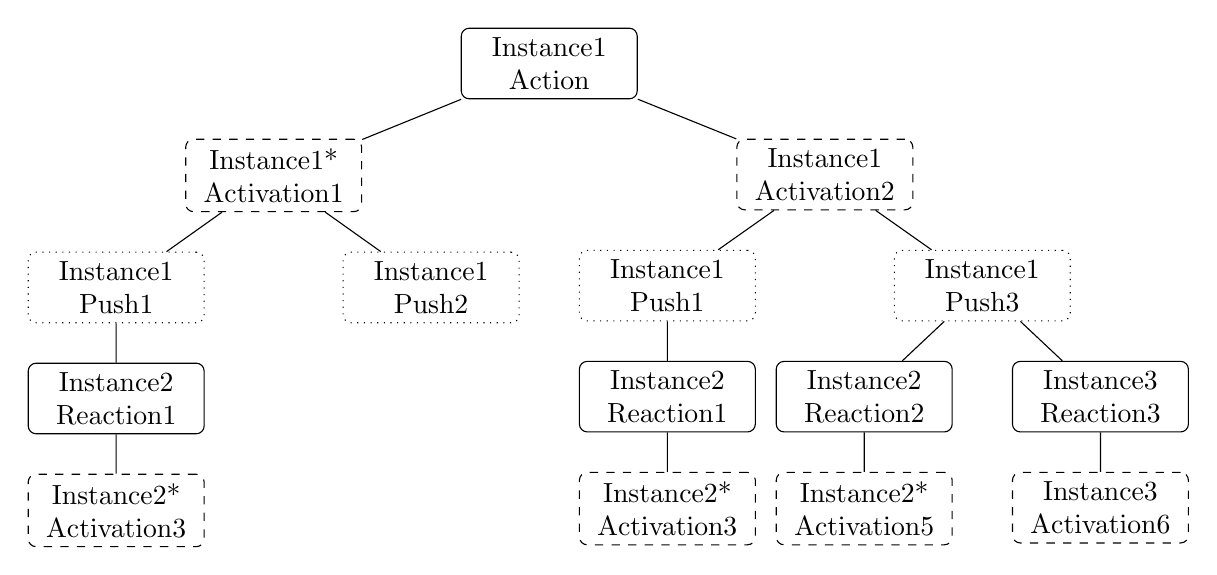
\begin{tikzpicture}[
    reaction/.style={rectangle, draw, rounded corners=1mm, text width=2cm,
        text centered, anchor=north},
    activation/.style={rectangle, draw, rounded corners=1mm, dashed, text width=2cm,
        text centered, anchor=north},
    push/.style={rectangle, draw, rounded corners=1mm, dotted, text width=2cm,
        text centered, anchor=north},
    level 1/.style={sibling distance=7.0cm},
    level 2/.style={sibling distance=4.0cm},
    level 3/.style={sibling distance=3.0cm},
    level distance=0.5cm, growth parent anchor=south
]
\node (Action) [reaction] {Instance1 Action}
  child {
    node (Activation01) [activation] {Instance1* Activation1}
    child {
      node (Push01) [push] {Instance1 Push1}
      child {
        node (Rection01) [reaction] {Instance2 Reaction1}
        child {
          node (Activation03) [activation] {Instance2* Activation3}
        }
      }
    }
    child {
      node (Push02) [push] {Instance1 Push2}
    }
  }
  child {
    node (Activation02) [activation] {Instance1 Activation2}
    child {
      node (Push04) [push] {Instance1 Push1}
      child {
        node (Rection08) [reaction] {Instance2 Reaction1}
        child {
          node (Activation08) [activation] {Instance2* Activation3}
        }
      }
    }
    child {
      node (Push03) [push] {Instance1 Push3}
      child {
        node (Rection02) [reaction] {Instance2 Reaction2}
        child {
          node (Activation04) [activation] {Instance2* Activation5}
        }
      }
      child {
        node (Rection03) [reaction] {Instance3 Reaction3}
        child {
          node (Activation05) [activation] {Instance3 Activation6}
        }
      }
    }
  }
;

\end{tikzpicture}
%%}%
\caption{Example concrete action\label{concrete_action}}
\end{figure}

\begin{figure}[H]
\centering
%%\resizebox{\textwidth}{!}{%
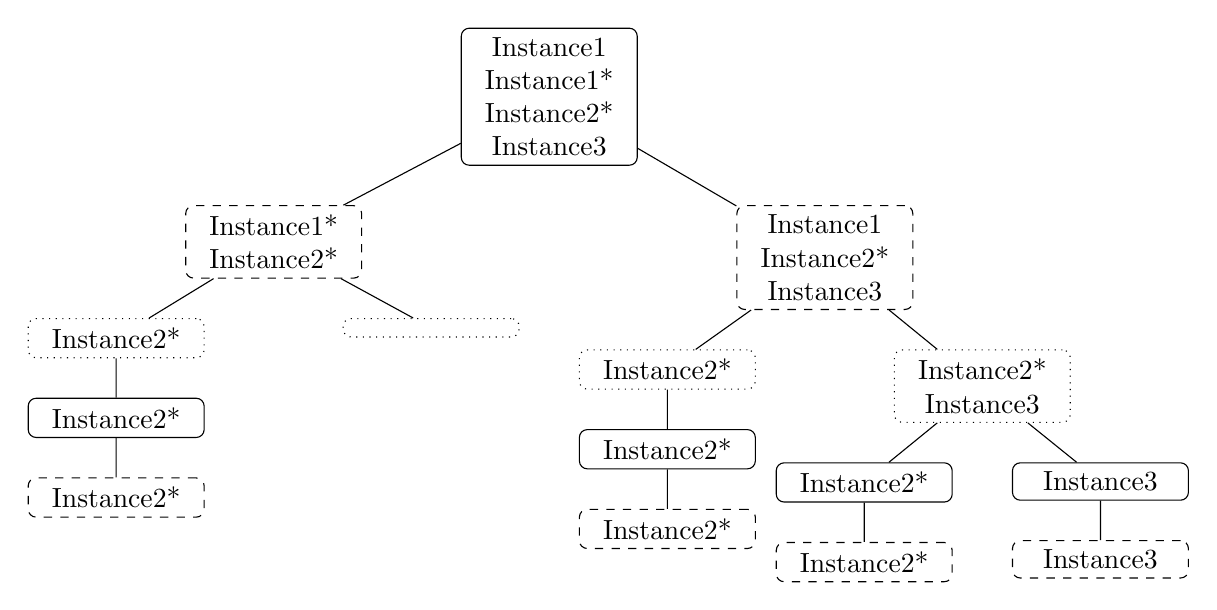
\begin{tikzpicture}[
    reaction/.style={rectangle, draw, rounded corners=1mm, text width=2cm,
        text centered, anchor=north},
    activation/.style={rectangle, draw, rounded corners=1mm, dashed, text width=2cm,
        text centered, anchor=north},
    push/.style={rectangle, draw, rounded corners=1mm, dotted, text width=2cm,
        text centered, anchor=north},
    level 1/.style={sibling distance=7.0cm},
    level 2/.style={sibling distance=4.0cm},
    level 3/.style={sibling distance=3.0cm},
    level distance=0.5cm, growth parent anchor=south
]
\node (Action) [reaction] {Instance1 Instance1* Instance2* Instance3}
  child {
    node (Activation01) [activation] {Instance1* Instance2*}
    child {
      node (Push01) [push] {Instance2*}
      child {
        node (Rection01) [reaction] {Instance2*}
        child {
          node (Activation03) [activation] {Instance2*}
        }
      }
    }
    child {
      node (Push02) [push] {}
    }
  }
  child {
    node (Activation02) [activation] {Instance1 Instance2* Instance3}
    child {
      node (Push04) [push] {Instance2*}
      child {
        node (Rection08) [reaction] {Instance2*}
        child {
          node (Activation08) [activation] {Instance2*}
        }
      }
    }
    child {
      node (Push03) [push] {Instance2* Instance3}
      child {
        node (Rection02) [reaction] {Instance2*}
        child {
          node (Activation04) [activation] {Instance2*}
        }
      }
      child {
        node (Rection03) [reaction] {Instance3}
        child {
          node (Activation05) [activation] {Instance3}
        }
      }
    }
  }
;

\end{tikzpicture}
%%}%
\caption{Example instance set calculation\label{instance_sets}}
\end{figure}

\paragraph{Enumerate concrete actions.}
Let $I$ be a component instance of type $T$.
Associated with $T$ is a set of actions $A$.
Each action $a \in A$ is evaluated for $I$ to create a concrete action.
A concrete action is a directed graph constructed as follows:
\begin{enumerate}
\item The root is $(I,a)$.
\item The descendants of the root are the activations in $a$.
\item The descendants of the activations are the push ports named in each activation.
\item The descendants of the push ports are the reactions bound to the push ports given by $reactions$.
\item This process is the repeated for each instance/reaction leaf.
\end{enumerate}
Figure~\ref{concrete_action} shows an example concrete action depicted as a tree.

The first step in analyzing a concrete action is to ensure that the directed graph is acyclic.
A cycle forms when a reaction activates itself through the set of concrete bindings.
Once the concrete action is proven free of cycles, it may be considered and represented as a tree as shown in figure~\ref{concrete_action}.
In the example, the Instance1/Push1 is activated by both Activation1 and Activation2.
It is replicated to convert the directed graph to a tree.

The second step in analyzing a concrete action is to determine which activations mutate the state of a component.
The current implementation uses a conservative static analysis of the body of an activate statement to determine if the activation mutates the state of the component.
These activations are marked with an asterisk (*) in figure~\ref{concrete_action}.

The third step is to compute a set of instances for each node in the concrete action.
If the node is not an activation, the set of instances is the union of the instances of its children.
If the node is an activation, the set of instances is the union of the instances of its children and the instance implied by the activation.
Figure~\ref{instance_sets} shows the instance set calculation for the concrete action in figure~\ref{concrete_action}.
The root shows that Instance1 does not change in at least one activation and may change in at least one activation, that Instance2 may change in every activation, and that Instance3 is ``read-only'' in this concrete action.

The fourth step is to check that a mutated instance appears in at most one child node instance set for the activation and push port nodes.
This check succeeds everywhere but Activation2 in figures~\ref{concrete_action}~and~\ref{instance_sets} as Instance2* appears in both children.
The activation and push port nodes represent activities that will be performed together.
That is, once control passes to an activation statement, all push ports and their bound reactions are activated.
In contrast, activations, as children of action and reaction nodes, represent mutually exclusive alternatives, i.e., at most one activation statement is executed per action/reaction body.
Thus, a mutated instance appearing in two or more children of an activation node or push port node indicates that the state of a component may be mutated in disparate ways leading to a non-deterministic state transition.

\section{BEGINNING OF UNADOPTED MATERIAL FROM PROPOSAL}

\paragraph{Compilation.}
To facilitate a design and development process based on composition and decomposition, we require a high-level language that resembles the model and examples presented in section~\ref{model}.
The goal of the compiler, then, is to translate the high-level language to the language of the $\alpha$-machine.
%% Complication typically consists of five phases corresponding to scanning, parsing, semantic analysis, optimization, and code generation.
In addition to conventional semantic analysis, e.g., type checking, the compiler will check that the reactive system is well-defined and provide a concurrency analysis to be used during scheduling.
%% Optimization is beyond the scope of this research.

Substitutional equivalence provides the logical foundation for testing well-definedness.
A system is represented as a top-level reactive component.
The input and output ports original to the top-level component can be converted to internal ports since the top-level component does not need an external interface.
Substitutional equivalence allows the declarations of member components to be replaced with their definitions according to the procedure outlined in section~\ref{model}.
This process can be repeated until all member components are ``inlined'' resulting in a top-level component that only contains state variables, internal ports, $\alpha$-statements, $\beta$-statements, and $\gamma$-statements.
At this point, all internal ports, $\gamma$-statements, and $\beta$-statements can be eliminated by substituting definitions.
The resulting top-level component only contains state variables and $\alpha$-statements.
To be a faithful implementation of the model, each $\alpha$-statement must be a deterministic state transformation.
The main challenge, then, lies in the co-design of a transformational language and checks for deterministic assignment.

At a high level, we desire to treat the transformation specified by an $\alpha$-statement as a function that maps a value representing the current state to a value representing the next state because it leads to a simple decidable check.
An $\alpha$-statement then consists of five parts:  a precondition list, a precondition function, an assignment list, an argument list, and an effect function.
The precondition list and argument list are lists of readable objects that form the arguments of the precondition function and effect function, respectively.
The assignment list is a list of writable objects that are assigned the values produced by the effect function (state variables that are not named in the assignment list retain their previous values and ports that are not named in the assignment list are undefined).
There is no notion of state or assignment inside the effect function, which thus resembles a pure functional or applicative program.
A conservative but decidable check, then, is to ensure that a writable object appears at most once in the assignment list.

%%Another concept implicit in the semantics of functional languages and their data structures is freedom from aliasing.
The approach outlined above hinges on the semantics of writable objects.
We define a writable object to be the name for an implied set of storage locations.
All elements in the set of storage locations for a scalar variable are updated in an assignment to the variable.
In contrast, only a subset of the set of storage locations for aggregate variables such as arrays and records may be updated in an assignment.
Variables can also name linked data structures where the set of locations is the transitive closure of a points-to analysis~\cite{hind2001pointer}.

For well-definedness, we require that the implied sets of storage locations for all writable objects be disjoint.
Thus, an assignment to two different variables in an $\alpha$-statement cannot update the same memory location.
The challenge then is to show that this condition holds initially and that it holds after the execution of each $\alpha$-statement.
This is the subject of pointer analysis~\cite{hind2001pointer} which is undecidable in general.
Components that communicate by passing data by reference as opposed to by value obviously violate this condition since multiple components may then reference the same memory locations.
Thus, data passed by reference through ports must have semantics that prevent concurrent updates, e.g., constant (read-only), copy-on-write, etc.
The goal then is to place appropriate restrictions on the language so as to make pointer analysis feasible and enable the safe sharing of data across ports.

To achieve the general approach outlined above, an approach to persistent data structures~\cite{driscoll1989making} and copy elimination~\cite{gopinath1989copy} is needed.
A persistent data structure is one in which updates and queries can be made to any version, e.g., lists in LISP, Scheme, Haskell, etc.
Persistent data structures match the semantics of existing functional programming languages since they allow variables to be treated as immutable values.
In contrast, an ephemeral data structure is one in which updates and queries can only be to the most recent version.
Ephemeral data structures are common in imperative languages and typically have simpler designs~\cite{okasaki1999purely}.
Copy elimination attempts to replace copying with in-place modification when it can be shown that the old value of a variable is no longer needed.
Copy elimination is often used for large aggregate data structures, e.g., arrays, that resist efficient persistent implementations.

An approach that to our knowledge has not been attempted is to restrict a functional language solely to ephemeral data structures.
We define an \emph{ephemeral function} to be a function with an implementation (i.e., \emph{schedule of operations}) that allows all data structures to be treated as ephemeral.
This approach has the potential to be more efficient since variables may be updated without copying.
Functions with no ephemeral schedule must explicitly introduce copying, which is beneficial since it makes the developer aware of such potentially costly operations.
Ephemeral functions may \emph{compose}, meaning that ephemerality may be established solely from the definition of a function and the signatures of any called functions.
The challenge then is to develop an analysis to determine if a function is ephemeral and design the language of $\alpha$-statement transformations based on this analysis.

The goal of concurrency analysis is to determine which $\alpha$-statements are independent and therefore can be executed concurrently.
Using the formulation above, we associate with each $\alpha$-statement a set of objects given by forming the union of the precondition list, assignment list, and argument list (called the $\alpha$-statement's \emph{implied objects}).
Two $\alpha$-statements are independent if their sets of implied objects are disjoint.

%% One idea is to treat $\alpha$-statements as ``pure'' data-flow programs which have properties that are conducive to analysis.
%% The structure present when compiling can also provide insights into the pointer analysis problem.
%% For example, one could envision a heap-per-component strategy where each heap is considered as an extra variable.
%% Passing a pointer through a port involves transferring the ownership of an object from one heap to another heap or set of heaps.
%% Thus, the language might include two pointer types corresponding to the pointers ability to be passed to another component.
%% This idea might be extended resulting in multiple heaps per component.

%% To be a faithful implementation of the model, each $\alpha$-statement must be a deterministic state transformation.
%% Thus, a compiler or verifier of $\alpha$-machine bytecode must be able to prove this property and the language of $\alpha$-statements must be designed around this constraint.
%% A conservative but straightforward approach to proving determinism for variables in static storage is to check that a state variable is written at most once in all possible executions of an $\alpha$-statement.
%% Existing techniques, e.g., control flow analysis, are adequate for this purpose.
%% Proving determinism for variables allocated on the heap requires pointer analysis, e.g., shape analysis~\cite{larus1988detecting}, an area of ongoing research.
%% Most likely, the language of $\alpha$-statements will need to be restricted to make pointer analysis feasible.

%% A compiler for this language takes as input reactive components constituting the system and uses the aforementioned techniques based on substitutional equivalence and simplification to produce an $\alpha$-machine program.
%% In addition to the aforementioned determinism check, the compiler should check for appropriate port usage, e.g., input ports are read while output ports are written, and port consistency (static versus dynamic).
%% The additional structure present when compiling from a high-level language will be useful when reporting errors related to non-deterministic assignment statements, perhaps by indicating the error using the same information presented in the block diagram of figure~\ref{clocksys_component_graphic} or the $\alpha$-forest diagram of \ref{clocksys_component_alpha}.
%% The compiler can also help in design as it can perform concurrency analysis which the developer might use to identify bottlenecks and reactive components or systems that are good candidates for redesign.


%% The $\alpha$-machine processes a low-level language similar to Java bytecode.
%% The reactive program given to an $\alpha$-machine lacks the structural elements, i.e., components, ports, $\beta$-statements, and $\gamma$-statements, needed to facilitate a design and development process based on composition and decomposition.

%% We believe that the gross structure for reactive components presented in the examples of section~\ref{model} is adequate for structuring systems.
%% The main challenge lies in the design of a transformational language that will facilitate the determinism checks.
%% One idea is to treat $\alpha$-statements as ``pure'' data-flow programs which have properties that are conducive to analysis.
%% The structure present when compiling can also provide insights into the pointer analysis problem.
%% For example, one could envision a heap-per-component strategy where each heap is considered as an extra variable.
%% Passing a pointer through a port involves transferring the ownership of an object from one heap to another heap or set of heaps.
%% Thus, the language might include two pointer types corresponding to the pointers ability to be passed to another component.
%% This idea might be extended resulting in multiple heaps per component.

%% A system is represented as a top-level reactive component.
%% Substitutional equivalence allows the declarations of member components to be replaced with their definitions according to the procedure outlined in section~\ref{formalization}.
%% This process can be repeated until all member components are ``inlined'' resulting in a top-level component that only contains state variables.
%% The input and output ports original to the top-level component can be converted to internal ports since the top-level component does not need an external interface.
%% At this point, all internal ports, $\gamma$-statements, and $\beta$-statements can be eliminated by substituting definitions.
%% The resulting top-level component only contains state variables and $\alpha$-statements.

%% \begin{figure}
%% {
%% \input workflow.tex
%% \centerline{\box\graph}
%% }
%% \caption{A compilation workflow for reactive components\label{workflow}}
%% \end{figure}

%% Figure~\ref{workflow} shows our proposed compilation workflow for reactive components.
%% The goal of the workflow is to transla

%% The workflow begins with the definition of the components and the designation (*) of one component as the top-level component that will represent the system.
%% Substitutional equivalence allows the declarations of member components to be replaced with their definitions according to the procedure outlined in section~\ref{formalization}.
%% This process can be repeated until all member components are ``inlined'' resulting in a top-level component that only contains state variables.
%% The input and output ports original to the top-level component can be converted to internal ports since the top-level component does not need an external interface.
%% At this point, all internal ports, $\gamma$-statements, and $\beta$-statements can be eliminated by substituting definitions.
%% The resulting top-level component only contains state variables and $\alpha$-statements.

%% The top-level component is then subjected to semantic analysis to determine if the system is well-defined.

%% The final step of compilation generates an $\alpha$-machine image which contains static allocated variables, executable code for realizing the $\alpha$-statements, and schedule analysis indicating which $\alpha$-statements can be executed concurrently.
%% The $\alpha$-machine image can then be instantiated to produce an executing instance of the reactive system.

\paragraph{$\alpha$-machine.}
We propose a virtual machine, called an $\alpha$-machine, capable of executing systems expressed as a single top-level component containing only state variables and $\alpha$-statements.
An $\alpha$-machine has five parts:
\begin{enumerate}
\item The \emph{data section} contains all of the statically allocated state variables.
\item The \emph{heap} contains dynamically allocated state variables.
\item The \emph{program} contains the code necessary to implement the $\alpha$-statements.
\item The \emph{stack} contains dynamic storage for function calls and expression evaluation.
\item The \emph{scheduler} selects and executes $\alpha$-statements.
\end{enumerate}
For simplicity, we will limit the design to a stack-based machine since code generation for stack-based machines is straightforward.
Our approach to dynamic allocation, garbage collection, etc. will be shaped by the transformational language used to encode $\alpha$-statements.


%% \paragraph{Program.}
%% To be a faithful implementation of the model, each $\alpha$-statement must be a deterministic state transformation.
%% Thus, a compiler or verifier of $\alpha$-machine bytecode must be able to prove this property and the language of $\alpha$-statements must be designed around this constraint.
%% A conservative but straightforward approach to proving determinism for variables in the data section is to check that a state variable is written at most once in all possible executions of an $\alpha$-statement.
%% Existing techniques, e.g., control flow analysis, are adequate for this purpose.
%% Proving determinism for variables allocated on the heap requires pointer analysis, e.g., shape analysis~\cite{larus1988detecting}, an area of ongoing research.
%% Most likely, the language of $\alpha$-statements will need to be restricted to make pointer analysis feasible.

%% \paragraph{Scheduler.}
Of primary interest to this research is the scheduler.
The scheduler selects $\alpha$-statements and executes them based on their preconditions.
Furthermore, the scheduler must be fair meaning that it cannot indefinitely postpone the selection of an $\alpha$-statement.
One way of measuring the efficiency of a scheduler is to compare the number of preconditions that evaluate to true to the total number of evaluated preconditions.
Similarly, one could measure the time spent evaluating and reevaluating preconditions to the time spent evaluating effects.
Schedulers can also be compared using other criteria such as responsiveness, fairness, cache-awareness, context-switches, etc.
%% Using the pointer analysis techniques outlined above, one can also analyze the relationships between $\alpha$-statements to determine which $\alpha$-statements are independent meaning that they operate on disjoint sets of state variables (read and write).
Independent $\alpha$-statements can be executed concurrently prompting the development of a concurrent $\alpha$-machine and concurrent schedulers.
A concurrent scheduler should take advantage of the static structure latent in reactive components and the dynamic behavior of the system being executed when making scheduling decisions.

%% \paragraph{Compilation.}
%% The $\alpha$-machine processes a low-level language similar to Java bytecode or assembly language.
%% The reactive program given to an $\alpha$-machine lacks the structural elements, i.e., components, ports, $\beta$-statements, and $\gamma$-statements, needed to facilitate a design and development process based on composition and decomposition.
%% Thus, to make developing reactive programs easier, we also require a high-level language that more closely resembles the model and examples presented in section~\ref{model}.
%% A compiler for this language takes as input reactive components constituting the system and uses the aforementioned techniques based on substitutional equivalence and simplification to produce an $\alpha$-machine program.
%% In addition to the aforementioned determinism check, the compiler should check for appropriate port usage, e.g., input ports are read while output ports are written, and port consistency (static versus dynamic).
%% The additional structure present when compiling from a high-level language will be useful when reporting errors related to non-deterministic assignment statements, perhaps by indicating the error using the same information presented in the block diagram of figure~\ref{clocksys_component_graphic} or the $\alpha$-forest diagram of \ref{clocksys_component_alpha}.
%% The compiler can also help in design as it can perform concurrency analysis which the developer might use to identify bottlenecks and reactive components or systems that are good candidates for redesign.

%% We believe that the gross structure for reactive components presented in the examples of section~\ref{model} is adequate for structuring systems.
%% The main challenge lies in the design of a transformational language that will facilitate the determinism checks.
%% One idea is to treat $\alpha$-statements as ``pure'' data-flow programs which have properties that are conducive to analysis.
%% The structure present when compiling can also provide insights into the pointer analysis problem.
%% For example, one could envision a heap-per-component strategy where each heap is considered as an extra variable.
%% Passing a pointer through a port involves transferring the ownership of an object from one heap to another heap or set of heaps.
%% Thus, the language might include two pointer types corresponding to the pointers ability to be passed to another component.
%% This idea might be extended resulting in multiple heaps per component.

\paragraph{Summary.}
In this section, we have proposed to implement the model described in section~\ref{model} for systems with static topologies.
We proposed to develop a virtual machine called an $\alpha$-machine that executes a reactive component consisting solely of state variables and $\alpha$-statements.
The $\alpha$-machine will be a concurrent $\alpha$-machine.
We also proposed to develop a high-level language for specifying reactive components and a compiler that translates the specifications into an $\alpha$-machine program.
The main challenge is the design of the high-level language, which must be subject to an analysis for deterministic assignment.

%% POSIX environment, possibly bare metal
